\begin{abstract}
FlexMAC compares precision adaptation with straightforward parallelism on a frozen ten-class digit classifier. An INT4-first engine uses conservative, input-conditioned score bounds to certify agreement with INT8, otherwise rerunning INT8. It certifies 351 of 359 calibration images, but its complete mapped implementation is larger and slower than a two-lane INT8 baseline. A subsequent register boundary separates completed-score comparison from accumulation. In a matched SKY130 typical-corner experiment, this change reduces no-gap latency from 5.220 to 4.448~$\mu$s at each design's directly tested passing period, with 1.493\% additional cell area. At a common 15~ns clock, its ten additional cycles instead increase latency by 2.604\%. These verified, pre-layout results demonstrate the importance of counting certificate hardware and clock-period costs; they establish neither energy savings nor production timing closure.
\end{abstract}
\begin{IEEEkeywords}
precision adaptation, quantization, RTL, conservative bounds, standard-cell mapping, static timing analysis
\end{IEEEkeywords}

\section{Introduction and Related Work}
The motivating question is whether lower precision remains useful after paying for preprocessing, buffering, decision certification, fallback, and control. A MAC-only comparison cannot answer that question. FlexMAC therefore progresses from a frozen classification workload to complete raw-input engines, characterized-cell mapping, mapped functional replay, and a timing-driven follow-up~\cite{flexmac}. This independent technical report consolidates those experiments without claiming peer review or algorithmic novelty. Its conference-template formatting does not imply publication or acceptance.

The contributions are an explicit agreement certificate with a bounded input domain; a verified full-engine comparison that rejects the current adaptive implementation's efficiency hypothesis; and a matched pipeline experiment that quantifies an area, cycle, and elapsed-time tradeoff. Negative results are retained alongside the improvement.

Bit Fusion composes bit-level processing elements to match varying DNN precision requirements~\cite{bitfusion}. It provides architectural context, rather than a directly comparable baseline for this small linear model. Dang et al. derive quantization-robustness guarantees using bilinear optimization and interval-bound methods~\cite{dang}. Their different method establishes relevant prior art for certified quantization. NVDLA illustrates the broader system scope of configurable CNN acceleration, including computation blocks, buffering, and memory interfaces~\cite{nvdla}. FlexMAC does not reproduce those systems or compare performance across their technologies.

\section{Frozen Workload and Conservative Agreement}
\subsection{Workload and Arithmetic Contract}
The workload uses the 1,797-image, $8\times8$ digits dataset distributed by scikit-learn~\cite{digits}. A project-specific stratified split with seed 20261027 assigns 1,078 training, 359 calibration, and 360 held-out images. Pixels are integers from 0 through 16. Multinomial logistic regression uses $C=1$, \texttt{lbfgs}, 3,000 maximum iterations, and tolerance $10^{-10}$. Calibration selects a global weight-clipping fraction separately for each precision. Integer weights, biases, split indices, scales, and fixtures are frozen~\cite{flexmac}.

\begin{table}[t]
\caption{Frozen classifier evaluation on 360 held-out images.}
\label{tab:accuracy}
\centering
\begin{tabular}{lrrr}
\toprule
Model & Correct & Accuracy & Drop \\
\midrule
Floating reference & 345 & 95.83\% & --- \\
INT8 & 345 & 95.83\% & 0.00 pp \\
INT4 & 341 & 94.72\% & 1.11 pp \\
\bottomrule
\end{tabular}
\end{table}

Table~\ref{tab:accuracy} shows that INT4 misses the predefined one-percentage-point budget. This finite sample does not establish a statistically significant accuracy difference. The adaptive and pipeline studies subsequently use the 359 calibration images; their replay and acceptance results are separate from held-out classification accuracy.

Each class score is a bias plus 64 signed products. Frozen preprocessing rounds ties to even after normalizing $p/8-1$. Scores use signed 32-bit wrap semantics. Exported absolute bounds of 223,820 for INT8 and 600 for INT4 establish that these frozen models cannot overflow, although directed arithmetic tests separately exercise the wrap contract.

\subsection{Input-Conditioned Residual Certificate}
Let $x_8(p)$ and $x_4(p)$ be the frozen preprocessing functions, and let $w_q(c,i)$ and $b_q(c)$ denote weights and biases at precision $q$. For raw pixels $p_i\in\mathcal{P}=\{0,\ldots,16\}$, define
\begin{equation}
S_q(c)=b_q(c)+\sum_{i=0}^{63}x_q(p_i)w_q(c,i).
\end{equation}
With positive scale $K=366$, the residual and bias difference are
\begin{align}
r(c,i,p)&=x_8(p)w_8(c,i)-Kx_4(p)w_4(c,i),\\
d(c)&=b_8(c)-Kb_4(c).
\end{align}
Condition the residual extrema on the observed INT4 bin $v$:
\begin{align}
m(c,i,v)&=\min_{\substack{p\in\mathcal{P}\\x_4(p)=v}}r(c,i,p),\\
M(c,i,v)&=\max_{\substack{p\in\mathcal{P}\\x_4(p)=v}}r(c,i,p).
\end{align}
For each observed $v_i=x_4(p_i)$, construct
\begin{align}
L(c)&=KS_4(c)+d(c)+\sum_{i=0}^{63}m(c,i,v_i),\\
U(c)&=KS_4(c)+d(c)+\sum_{i=0}^{63}M(c,i,v_i).
\end{align}
Every actual residual belongs to its conditioned interval. Summing those inequalities and using
\begin{equation}
S_8(c)=KS_4(c)+d(c)+\sum_{i=0}^{63}r(c,i,p_i)
\end{equation}
proves $L(c)\leq S_8(c)\leq U(c)$. Accept an INT4 candidate $c$ only if
\begin{equation}
L(c)>U(j)\quad\text{for every }j\ne c.
\label{eq:accept}
\end{equation}
Strict separation ensures the unique INT8 winner. This certifies agreement with the frozen INT8 classifier, not correctness against the digit label. Failed certification triggers exact INT8 evaluation. The mathematical argument assumes supported raw pixels, unchanged models, and correct arithmetic and control; it is not a formal verification of the RTL.

\section{Architectures and Register Placement}
All compared raw-input engines accept 64 five-bit pixels through ready/valid handshakes and retain the frame for computation. Verilog lookup tables implement frozen preprocessing. Pixels above 16 produce an input error after collection. Synchronous reset cancels the transaction; results remain stable under backpressure. Loading and evaluation do not overlap, and a new command waits until the current result is consumed~\cite{flexmac}.

Single-lane INT8 evaluates 640 products after 64 loading cycles, giving 704 command-to-valid cycles without gaps. Two-lane INT8 evaluates two products per cycle, taking 320 evaluation cycles and 384 cycles overall. Both calculate identical frozen INT8 scores and choose the lowest class index on ties.

The adaptive variants first evaluate packed INT4 while accumulating residual lower and upper bounds. A ten-cycle checker either accepts the INT4 candidate or starts a 640-cycle INT8 rerun from retained raw pixels. Certified frames take 394 cycles; fallbacks take 1,034. Shared and mux variants differ in their configurable product implementation. The residual table contains 9,600 used combinations with two 13-bit bounds each, or 249,600 logical bits before synthesis. This is representation size, not silicon area. Mapped cost includes ROM logic, intervals, quantization, arithmetic, and control.

\begin{figure*}[t]
\centering
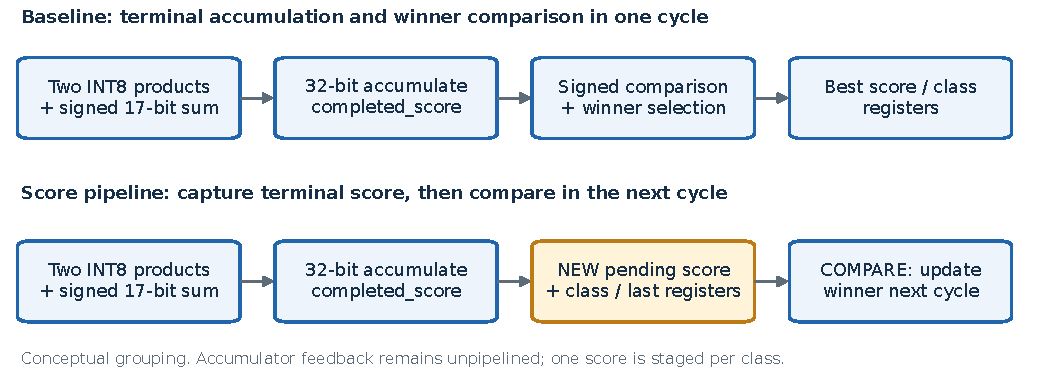
\includegraphics[width=\textwidth]{report_datapath.pdf}
\caption{Conceptual raw-input engine organization and completed-score register boundary, derived from the FlexMAC RTL~\cite{flexmac}. The diagram explains functional structure; it is not a routed layout or an extracted gate schematic.}
\label{fig:datapath}
\end{figure*}

The follow-up targets the two-lane baseline's measured path through accumulation and best-score comparison (Fig.~\ref{fig:datapath}). It registers the completed class score and class tag, then compares in an explicit subsequent state. The accumulation feedback loop still accepts one product pair per evaluation cycle: the new register is at the completed-score boundary. Ten comparison states increase the schedule from 384 to 394 cycles. Raw inputs, weights, quantization, signed arithmetic, and tie behavior remain unchanged.

The original host-quantized fixed INT4 interface takes 352 cycles, including 32 packed input bytes. It excludes host quantization and has neither raw-input checking nor the adaptive certificate. Comparing that count directly with the raw adaptive engine's 394 cycles would mix interface and functionality costs.

\section{Verification and Mapping Methodology}
\subsection{Functional Checks and Replay Coverage}
RTL regression checks frozen class scores and predictions, interval containment, certificate decisions, exact cycle counts, input gaps, output stalls, invalid pixels, and reset cancellation. The pipeline bench additionally checks pending class tags, comparison-state resets, and final-class publication. Directed tests cover signed ties and arithmetic/control corner cases. These tests support implementation correctness without constituting formal equivalence.

Mapped replay uses executable zero-delay models expanded from library Boolean and flip-flop functions. In the original four-design study, both INT8 engines replay all 359 calibration frames in Verilator 5.020 two-state simulation and Icarus 12.0 four-state simulation. Each adaptive engine replays all 359 frames in two-state simulation, but only 18 in four-state simulation: all eight fallbacks and one certified example for each of ten predicted classes. This subset followed a full adaptive Icarus attempt exceeding its time limit. In the separate pipeline study, both the pipeline variant and matched two-lane baseline replay all 359 frames in both simulators. Mapped checks compare outputs, flags, and cycles; internal score checks belong to RTL regression~\cite{flexmac}.

\subsection{Cell Mapping and Timing Model}
Yosys 0.33 performs flattened synthesis, flip-flop mapping, and Liberty-based ABC mapping with a 10~ns optimization target~\cite{yosys}. OpenSTA 3.1.0 analyzes a pinned SKY130 high-density library at typical process, $25\,^{\circ}$C, and 1.80~V~\cite{opensta,sky130}. Characterized cell areas are summed; these are not placed core areas. Library wire-load defaults are removed to make ideal wires explicit.

Every design uses ideal clocks, 0.10~ns clock transition, 0.10~ns setup uncertainty, zero hold uncertainty, external input/output maximum delays of $0.2$ times the tested period, zero minimum delays, \texttt{buf\_2} input driving, and 10~fF output loads. Synchronous reset is timed. There are no false or multicycle paths.

Repeated complete timing runs bisect a failing/passing setup bracket to at most 0.05~ns. Passing endpoints are directly tested with regenerated external budgets. Common periods round 110\% of the largest passing endpoint upward to 0.5~ns: 19~ns for four designs, 15~ns for the pipeline pair. All designs fail the 10~ns target. Reported no-gap latencies exclude injected input gaps, result-consumption stalls, and idle turnaround.

\subsection{Archived Evidence}
Original mapping results correspond to source revision \href{https://github.com/jrmywm/FlexMAC/commit/96141e7767723cfd53e6830a948e46bef05687d8}{\texttt{96141e7}} and \href{https://github.com/jrmywm/FlexMAC/actions/runs/40475813403}{run 40475813403}. Pipeline results correspond to \href{https://github.com/jrmywm/FlexMAC/commit/8e9065cb147d38b66423997e6d960a7239d8f5e9}{\texttt{8e9065c}} and \href{https://github.com/jrmywm/FlexMAC/actions/runs/40613482958}{run 40613482958}. The repository archives comparison CSVs, replay records, timing constraints, and provenance under \texttt{docs/data/mapping} and \texttt{docs/data/scorepipe}~\cite{flexmac}.

\section{Measured Results}
\subsection{Complete-Engine Comparison}
Table~\ref{tab:engines} reports the archived four-design experiment. Mean adaptive cycles weight 351 certified frames and eight fallbacks; they describe the calibration replay distribution:
\begin{equation}
\overline{N}=\frac{351(394)+8(1034)}{359}=408.2618\ldots.
\end{equation}
Two-lane INT8 beats both adaptive implementations despite their 97.77\% certification rate. Adaptive cell area is approximately 5.6 times the baseline area, and even certified frames exceed the two-lane baseline's cycle count. At the common 19~ns period, adaptive mean latency remains above two-lane INT8. The complete-engine evidence overturns the favorable impression from acceptance rate alone.

\begin{table*}[t]
\caption{Original four-design raw-input comparison from archived mapped results~\cite{flexmac}. Own-period latency uses each row's directly tested passing endpoint. Common-period latency uses 19~ns. Adaptive averages cover 359 calibration images; areas are characterized cell-area sums before layout.}
\label{tab:engines}
\centering
\begin{tabular}{lrrrrr}
\toprule
Raw-input engine & Area ($\mu$m$^2$) & Pass (ns) & Cycles mean / worst & Mean own ($\mu$s) & Mean common ($\mu$s) \\
\midrule
Single-lane INT8 & 26,357.78 & 11.7578125 & 704 / 704 & 8.278 & 13.376 \\
Two-lane INT8 & 30,006.28 & 13.5937500 & 384 / 384 & 5.220 & 7.296 \\
Adaptive shared & 167,946.07 & 17.0312500 & 408.26 / 1,034 & 6.953 & 7.757 \\
Adaptive mux & 167,561.96 & 17.1875000 & 408.26 / 1,034 & 7.017 & 7.757 \\
\bottomrule
\end{tabular}
\end{table*}

\subsection{Matched Pipeline Experiment}
The separate matched experiment reproduces the baseline's exact netlist hash, area, and timing bracket before evaluating the new boundary. Table~\ref{tab:pipeline} reports the pair. The pipeline saves 14.791\% own-period latency for 1.493\% additional cell area, adding 38 sequential cells. At a common 15~ns period it is 2.604\% slower. Thus its benefit depends on exploiting the shorter feasible clock, as summarized in Fig.~\ref{fig:results}.

\begin{table}[t]
\caption{Matched two-lane comparison. Latencies exclude gaps and stalls.}
\label{tab:pipeline}
\centering
\begin{tabular}{lrr}
\toprule
Metric & Baseline & Registered \\
\midrule
Cell area ($\mu$m$^2$) & 30,006.2784 & 30,454.2080 \\
Passing period (ns) & 13.5937500 & 11.2890625 \\
Cycles & 384 & 394 \\
Own-period latency ($\mu$s) & 5.220000 & 4.447891 \\
Latency at 15 ns ($\mu$s) & 5.760 & 5.910 \\
\bottomrule
\end{tabular}
\end{table}

\begin{figure*}[t]
\centering
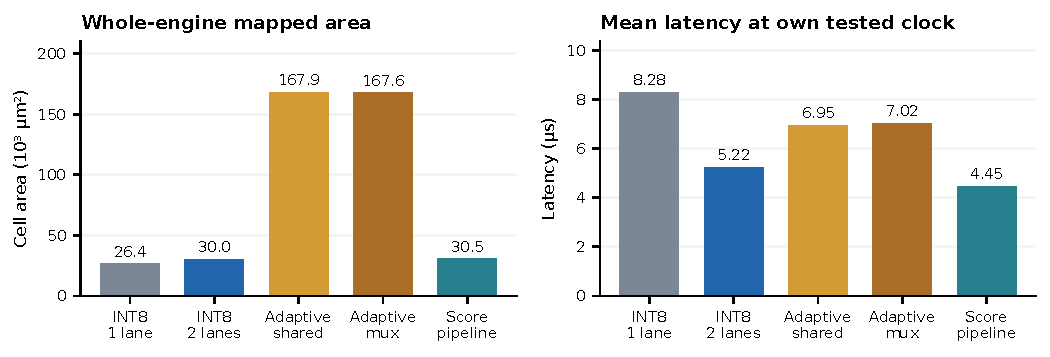
\includegraphics[width=\textwidth]{report_results.pdf}
\caption{Mapped complete-engine comparison and matched pipeline tradeoff, plotted from the archived comparison CSVs~\cite{flexmac}. Areas and timing are pre-layout SKY130 typical-corner results under ideal-wire and ideal-clock assumptions. Adaptive means use the 359-image calibration distribution; these plots are not energy or silicon measurements.}
\label{fig:results}
\end{figure*}

The reported worst endpoint changes from \texttt{best\_score[0]} to \texttt{accumulator[30]}, consistent with separating score comparison from accumulation. The measured result supports this boundary placement, not an unmeasured further optimization.

\section{Limitations and Conclusion}
Precision reduction creates opportunity only when its supporting machinery costs less than the work saved. Here, a high certificate acceptance rate does not compensate for residual-table logic and a slower complete engine. Straightforward INT8 parallelism is the stronger original design; registering its score comparison then improves elapsed time under the stated timing model.

Passing setup slacks at the matched endpoints are only $+0.002972$~ns and $+0.005231$~ns. These tiny positive margins reflect discrete search resolution, not practical signoff margin. Common-clock setup and hold pass with no reported maximum-slew or capacitance violations, but ideal-clock hold checks do not establish clock-tree closure. Replay has no SDF and does not measure physical timing or glitches.

The evidence covers one linear model and one typical library corner. It includes no placed-and-routed implementation, measured power, energy, FPGA result, SoC integration, or formal proof of RTL correctness. Calibration-based architecture exploration provides no new held-out accuracy evidence. Broader workloads, independent evaluation, and physical implementation would be needed before generalizing. Within this boundary, FlexMAC provides a reproducible example of rejecting an expensive adaptation strategy and validating a conventional pipeline change with explicit tradeoffs.
